
\chapter{Literature Review}\label{Ch:2}
\vspace{30pt}


\section{Stroke}\label{sec:Stroke}
\subsection{What is Stroke?}\label{stroke?}
Stroke can be defined in general as \begin{quotation}
	
	“\textit{an episode of acute neurological dysfunction presumed to be caused by Ischemia or Haemorrhage, persisting for more than 24 hours or until death, but without any sufficient evidence to be classified as one of the above.”}\\
	\begin{flushright}
		\cite{Sacco2013}
	\end{flushright}
\end{quotation}
This is the new updated definition which also describes other definitions of stroke based on the causes which are listed below. 
\begin{itemize}%typesof strokes
	\item \textbf{Ischemic stroke}: an episode of neurological dysfunction caused by focal cerebral, spinal, or retinal infraction.
	\item \textbf{Stroke cause by intracerebral haemorrhage}: this is when clinical signs of neurological dysfunction that are related to a focal point in the brain rapidly develop, and it is not caused by trauma.
	\item \textbf{Stroke caused by subarachnoid haemorrhage}: this is a stroke that is associated with neurological dysfunction and/or headache because of bleeding into the subarachnoid space and is not cause by trauma.
	\item \textbf{Stroke caused by cerebral venous thrombosis}: this stroke can be described as an infraction or haemorrhage in the brain, spinal cord, or retina because of thrombosis of the \ac{cvs}. 
\end{itemize}

\subsection{Stroke Classification}
Since stroke is a disabling disorder, and it is the leading cause of disability in the world. The effects can be classified under the \ac{who}'s international classification of function, disability and health \cite{Stucki2005}.\\
\cite{mayosym} Based on the cause of stroke, there are 3 classifications which are listed below:
\begin{itemize}%classification list
	\item \textbf{Ischaemic Stroke}: which results for about 80\% of all strokes.
	\item \textbf{Haemorrhagic stroke}: which results for about 15\% of all strokes causes and is subdivided into 2 which are:
	\begin{itemize}
		\item Intracerebral which accounts for 10\%
		\item Subarachnoid that accounts for 5\%
	\end{itemize}
	\item \textbf{Not specified}: results for 5\% of strokes
\end{itemize}
In terms of getting a Diagnosis for stroke there are many methods that can be used \cite{mayodiag}, but the most used for Diagnosis and examinations are:
\begin{itemize}%diagnosis list
	\item \ac{ct} or \ac{mri} scan (with and without contrast)
	\item Doppler
	\item An \ac{eeg} session with a induced reaction.
	\item \ac{ecg}
	\item History of patient and family
	\item Clinical examination
	\item Fundoscopic examination
	\item Auscultation
	\item Blood analysis
\end{itemize}
Stroke can affect any part of the human body, and the effects of those parts being affected can result in catastrophic results, the most relevant structures that can be affected by stroke are:
\begin{itemize}%locations affected list
	\item The brain shown in Figure \ref{fig:brain}.
	\item Cardiovascular system
	\item Leg and arm: the sites of most stroke related disabilities
	\item Shoulder region
\end{itemize}
Stroke also affects body functions and activities as well as body structures, The Body structures affected by a Stroke and the influence on the activities are shown in Figure \ref{fig:effects}.

\begin{figure}[p]%figure types
	\centering
	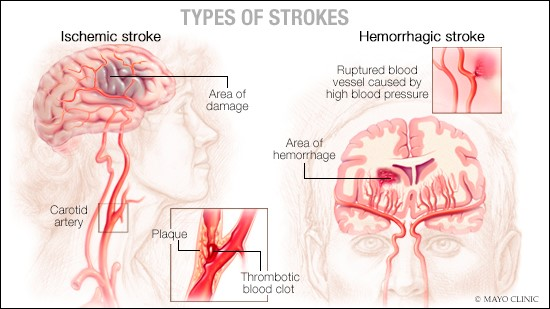
\includegraphics[width=1.1\linewidth]{figures/ch2/strokecauses}
	\caption{Figure showing the causes and Main types of stroke \cite{mayostroke}.}
	\label{fig:brain}
\end{figure}

\begin{figure}[p]%figure effects
	\centering
	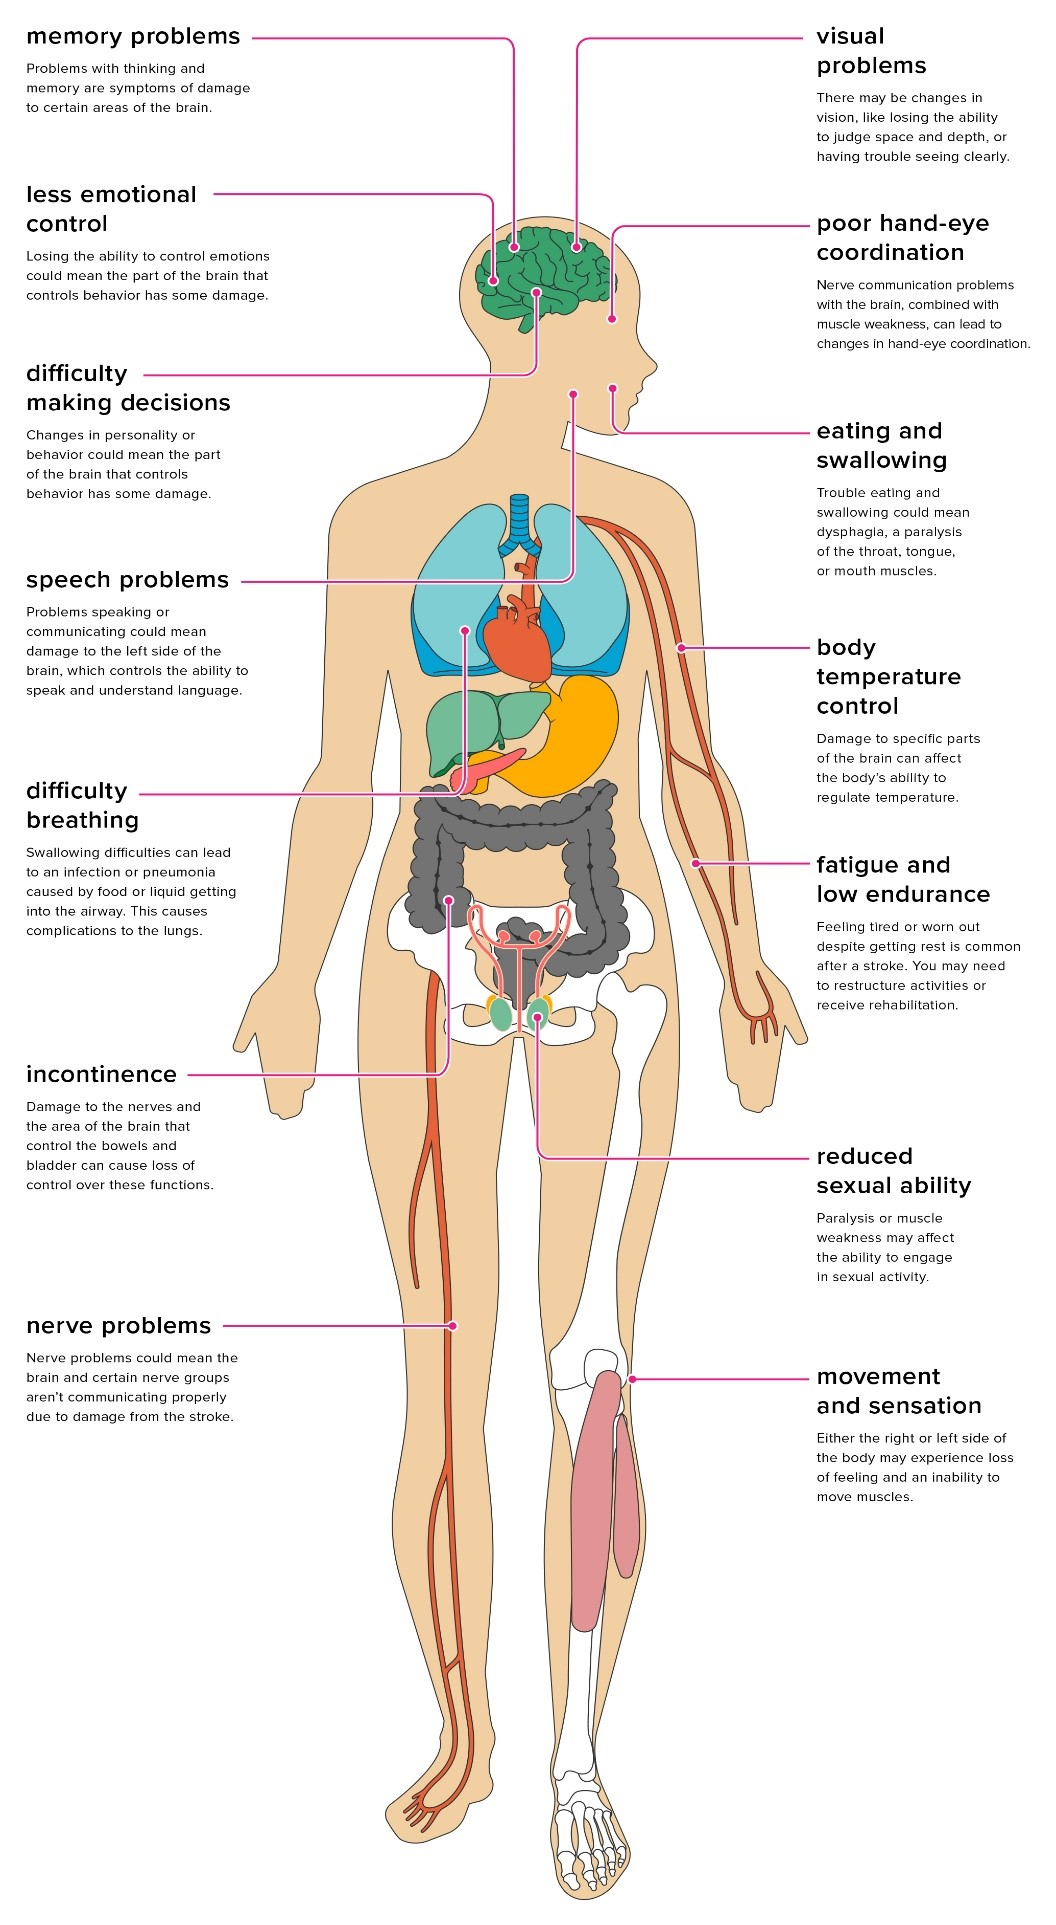
\includegraphics[height=22cm]{figures/ch2/strokeeffects}
	\caption{Figure showing the effects on the body from Stroke \cite{Marcin2019}.}
	\label{fig:effects}
\end{figure}
\newpage

\subsection{Stroke Symptoms}
Since Stroke is a medical emergency, early recognition of its symptoms can help in prompt treatment for such patients, \cite{mayosym} the signs that a person is experiencing a stroke include:
\begin{itemize}%symptoms list
	\item \textbf{Trouble speaking and understanding what others are saying.} 	 There might be an experience of confusion, slurring of words or having a difficulty understanding speech.
	\item \textbf{Paralysis or numbness of the face, arm and leg.} There might be a development of sudden numbness, weakness or paralysis in the face, arm or leg, this often affects only one side of the body. A way to test for this is for the person to raise both their arms above their head and if one arm begins to fall it means the person in question might have a stroke.
	\item \textbf{Problems seeing in one or both eyes.} Sudden blurred or blackened vision in one or both eyes, and seeing double
	\item \textbf{Headache.} A sudden headache accompanied by vomiting, dizziness or altered consciousness may indicate stroke
	\item \textbf{Trouble walking.}  When walking and you stumble or lose one’s balance, there may also be sudden dizziness or loss of coordination.
\end{itemize}

If any of the signs have been noticed there is also a check for being sure of the symptoms and it is known as “FAST”\\
\begin{itemize}%fast list
	\item[\textbf{F:}]\textbf{ Face.} Ask the person to smile, does one side of the face droop?
	\item[\textbf{A:}]\textbf{ Arms.} Ask the person to raise both arms. Does one arm drift downward? Or is one arm usable to rise.
	\item[\textbf{S:}]\textbf{ Speech.} Ask the person to repeat a simple phrase, is his or her speech slurred or strange.
	\item[\textbf{T:}]\textbf{ Time.} If you observe any of these signs call emergency medical help immediately.
\end{itemize}


\subsection{Stroke Risk Factors }
There are many factors that can increases a person’s stroke risk, they can be divided into lifestyle risk factors, medical risk factors and other factors \cite{mayostroke}.\\
Lifestyle risk factors are factors external to the body that a person indulges in that can increase their stroke risk, While Medical risk factors are those which originate from the body, can be innate or through sickness. examples of lifestyle and medical risk factors are:
\begin{itemize}%lifestyle & medical risk factorss
	\item[] Physical inactivity
	\item[] Heavy drinking or binge drinking
	\item[] Use of illegal drugs
	\item[] Cardiovascular disease
	\item[] Family history of stroke, heart attack or transient ischemic attack 
\end{itemize}



\subsection{Stroke Complications}
A stroke can sometimes cause temporary or permanent disabilities depending on how long the brain lacks blood flow and which part was affected. Complications may include the following and they are also indicated in Figure \ref{fig:effects}:
\begin{itemize}%complications list
	\item Paralysis or loss of muscle movement. a person may be paralyzed if the part of the brain responsible for the movement of that limb is affected.
	\item Difficulty talking or swallowing. A stroke may affect control of the muscles in the mouth and throat resulting in difficulty talking, swallowing and eating. There can also be difficulty with language including speaking or understanding speech, reading or writing.
	\item Memory loss or thinking difficulties. Many people who have had stroke experience some memory loss. Others may have difficulty thinking, reasoning, making judgements and understanding concepts.
	\item Emotional problems. People who have had stroke may have more difficulty controlling their emotions, or they may develop depression.
	\item Pain. Pain, numbness or other unusual sensations may occur in the parts of the body affected by stroke.
	\item Changes in behavior and self-care ability. People who have had stroke may become more withdrawn. They may need help with grooming and daily chores.
\end{itemize}

\subsection{Stroke Recovery and Rehabilitation}
After emergency treatment patients are usually monitored for at least a day, after which stroke care in then focused on helping the patient recover as much function as possible so the patient can return to independent living. The impact on the brain from stroke depends on the area of the brain involved and the amount of tissue damaged, if the stroke affected the right side of the brain, movement and sensation on the left side may be affected and same for the left side of the brain and the right side of the body. And brain damage to the left side of the brain can cause speech and language disorders. \\
The Stroke rehabilitation process can be described as a cycle that involves: assessment of the patient’s needs, goal setting for improvement, intervention to assist with said goals, and reassessment at some periodic time to assess the progress towards the goal. \cite{mayostroke,eggers1984occupational}\\
The future effect of stroke on a patient is dependent on the site and size of the initial stroke lesion and the extent of the recovery. Recovery is through a combination of learning-dependent processing that included restitution, substitution, and compensation. Even though stroke recovery is unique the recovery in the first days are predictable \cite{Langhorne2011a}. Therefore, it is important to start the recovery process to allow for large gains in functional ability, shown in Figure\ref{fig:recovery}.

\begin{figure}[p]%figure of recovery curve
	\centering
	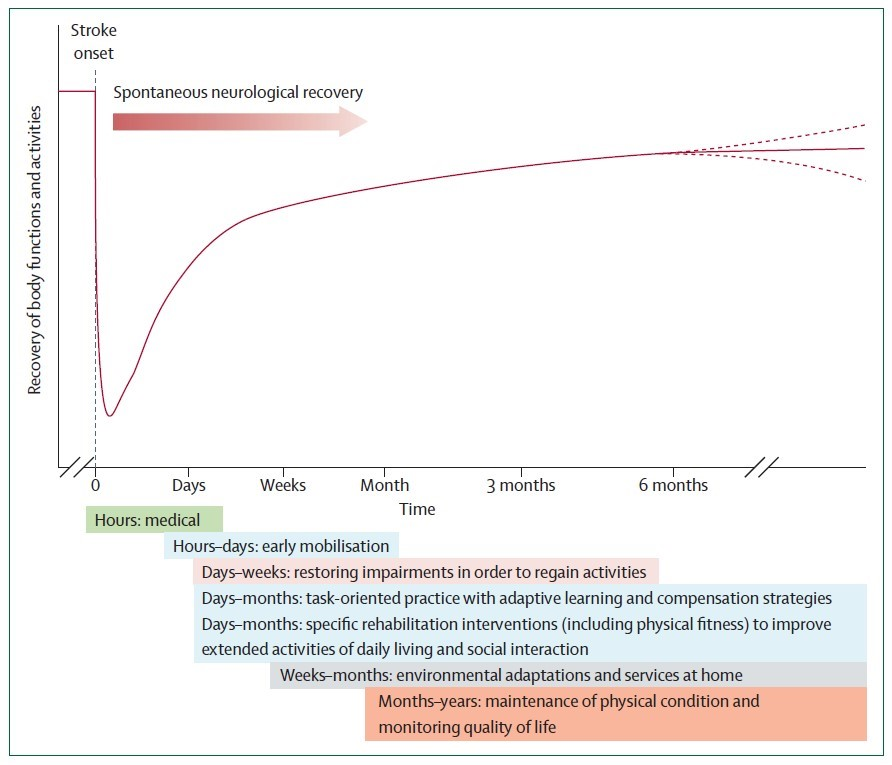
\includegraphics[width=14cm,height=10cm]{figures/ch2/recpattern}
	\caption{A figure showing the hypothetical pattern of recovery after stroke with timing of intervention strategies \cite{Langhorne2011a}.}
	\label{fig:recovery}
\end{figure}
\newpage
\section{Rehabilitation Robots}\label{sec:rehabrobots}
\subsection{What is Rehabilitation}
Rehabilitation can be defined as \begin{quotation}
	\textit{``a set of interventions designed to optimize functioning and reduce disability in individuals with health conditions in interaction with their environment''}\\
	\begin{flushright}
		\cite{Sjolund2013}
	\end{flushright}
\end{quotation}.
Rehabilitation as described by Eggers \cite{eggers1984occupational}, says that the end goal of rehabilitation should not only be the conscious use of the paralysed hand. But the end goal should be to allow the paralysed hand to be able to person some of the tasks it used to do before paralysis\cite{Johnson2005}.\\
As listed in \cite{whorehab} some examples of rehabilitation include : 
\begin{itemize}%examples of rehabilitation
	\item Exercises to improve a person’s speech, language and communication after a brain injury.
	\item Modifying an older person’s home environment to improve their safety and independence at home and to reduce their risk of falls.
	\item Exercise training and education on healthy living for a person with a heart disease.
	\item Making, fitting and educating an individual to use a prosthesis after a leg amputation.
	\item Positioning and splinting techniques to assist with skin healing, reduce swelling, and to regain movement after burn surgery.
	\item Prescribing medicine to reduce muscle stiffness for a child with cerebral palsy.
	\item Psychological support for a person with depression.
	\item Training in the use of a white cane, for a person with vision loss.
\end{itemize}

\subsection{Stroke Rehabilitation}
From literature it has been found out that most of the upper limb rehabilitation therapies done are only 50\% efficient \cite{Johnson2003}, however it has also been shown in other studies that the recovery process can be improved through forced use and enhanced therapy \cite{Duncan1997}.\\
What both forced use and enhanced therapy have in common is active participation, increased practise time, increased involvement and more repetitive training \cite{Johnson2003}.This means after a stroke, a patient will typically lose a lot of their functional ability, and the best time for gaining back that ability is within the first 6 months before the stroke is considered chronic. And with task-specific training, or other methods like high-intensity training, repetitive task training and through the use of robotics to assist in the rehabilitation \cite{Dobkin2004,Langhorne2011}.\\
Rehabilitation is highly patient specific, implying that each patient with a particular form of disability must have a rehabilitation intervention and approach designed for their goals and preferences and on the magnitude of the disability.

\subsection{Rehabilitation Robots}
The process of rehabilitation involves 4 steps as listed in \cite{Laut2016}, which are to access the type and extent of impairment, set goals to direct treatment and plan intervention to meet the goals, implementing the intervention,and reassessing the impairment level after intervention, and this steps are repeated till a impairment level is reached that is acceptable by the patient.\\
Rehabilitation robots can be used to enhance any of the steps listed above. Based on Intervention the robot can be designed to intervene in a specific region of the body, Upper limbs or lower Limbs \cite{Laut2016}.Rehabilitation robots can be divided into those that help to train (robot-aided therapy), support (exoskeleton) and replace (prosthesis) impaired activities or body functions and structures. \\
Due to the shortage of therapists to perform rehabilitation there is a need for intervention in the form telerehabilitation or advanced rehabilitation robots, which are expected to assist patients to complete therapy as accurate as well as conventional methods \cite{Sheng2016}.

\subsection{Classification of Rehabilitation Robots}
There are various ways to categorize the types of rehabilitation robots, the most classification types are from \cite{Sheng2016} and a literature review carried out personally with some of the results shown in tables: \ref{tab:reviewbilateral} and \ref{tab:reviewclincal}.\\
Based on the impairment location target for intervention, rehabilitation robots can be categorized as:
\begin{itemize}%rehab robots location aim
	\item \textbf{Lower extremity rehabilitation robots}: these are rehabilitation robots for the lower extremity of the body e.g., the legs, robots for gait.
	\item \textbf{Upper extremity rehabilitation robots}: these are rehabilitation robots for the upper extremity of the body, such robot types are: hand orthosis, upper arm rehab robots, full arm exoskeletons. 
\end{itemize}
The robot in this study is a Upper extremity rehabilitation robot, this category of robots can further be classified into 3 based on the impairment location in the upper arm \cite{Sheng2016}, these classifications are: 
\begin{itemize}%upper limb classification
	\item \textbf{Hand rehabilitation robots}: these are robots that are designed to help patients recover hand movement functions such as: grasping and grabbing. They usually coexist with Arm rehabilitation robots \cite{Troncossi2016}.
	\item \textbf{Arm Rehabilitation robots}: these robots are designed to rehabilitate the Upper arm, and can either rehabilitate the whole arm together, like the \ac{ulexo} (shown in Figure:\ref{fig:ulexo}) \cite{Shen2019a,Simkins2016}.
	\item \textbf{In-clinic devices for Occupational and physical therapy}: these types of robots are made to help patients in their rehabilitation process at their home without the need to visit a specialist, one type of robot in this category is a telerehabilitation robot/system \cite{Song2016,Carignan2006,Laut2016,Sheng2016}.
\end{itemize}
Robots that perform their tasks effectively have means to interact with their environment to perform and complete their tasks, for rehabilitation robots they need to have a connector that allows them to move the patients limbs to allow for rehabilitation of the muscles, based on this methodology there are 2 methods of patient robot interaction for Upper limb rehabilitation robots which are:
\begin{itemize}%human interaction
	\item \textbf{End-effector systems}: these are system that have an end effector (usually a handle), that the patient holds to interact with the robot. These only control from the contact area, usually the hands and require complex algorithms to be able to accurately control the movement of arm along the required path. There are other forms of interaction though games and VR. Examples of Robots like this are the \ac{mime} and \ac{arcmime} \cite{Mahoney2003,OMalley2006}, the \ac{biadler} (shown in Figure: \ref{fig:biadler}) \cite{Lott2016,Johnson2011b}, and others.
	\item \textbf{Exoskeleton systems}: these are systems whose mechanisms  cover the body part to be rehabilitated and they control the precise movement unlike the end-effector systems but they can be dangerous on the patient if not accurately designed and tested. Examples are  \ac{ulexo} (shown in Figure \ref{fig:ulexo}) \cite{Kim2013,Simkins2016}, and the HARMONY rehabilitation robot \cite{Kim2017}.
\end{itemize}
Rehabilitation robots, like all other robots have to perform their functions within a specified region which is called their workspace, based on this definition rehabilitation robots can be classified based on the type of workspace they operate in, there are 2 types of workspace that have been used by rehabilitation robots so far \cite{Sheng2016}, these classifications are:
\begin{itemize}%rehab robot task area
	\item \textbf{Planar workspace}: This workspace describes a robot only being able to act along a line or on a square on a table. The robots that use this workspace types are simple in design, thus the reason there are more commercial planar robots available like the \ac{bmt} (shown in Figure:\ref{fig:bmt}) \cite{Hesse2006,Hsieh2016,Schmidt2004}, and the MIT-MANUS \cite{Hesse2003,Hogan1992,Waldner2009}. Which are some of the more popular robots. 
	\item \textbf{3D workspace}: This workspace describes the robot being able to move the subjects arm in any of the 3 Cartesian coordinates along the length the arm can move, this workspace is versatile as it is able to allow the robot to perform many daily tasks compared to the planar workspace. With this workspace the patient can practice eating tasks, drinking, carrying a cup and much more. Examples of robots that use this type of workspace are the \ac{arcmime} \cite{Mahoney2003},\ac{built} \cite{Sampson2012a}),\ac{ulexo} (shown in Figure:\ref{fig:ulexo}) \cite{Shen2019a,Simkins2016}.
\end{itemize}
\begin{figure}[p]%bimanu image
	\centering
	
	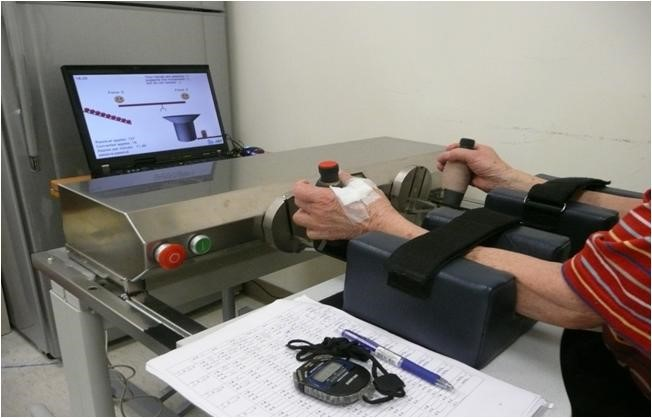
\includegraphics[width=\linewidth]{figures/ch2/bimanu}
	\caption{Picture showing a patient using the \ac{bmt}. \cite{bimanuimage}.}
	\label{fig:bmt}
\end{figure}

\begin{figure}[p]%biadler image
	\centering
	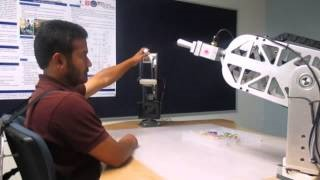
\includegraphics[width=\linewidth]{figures/ch2/biadler}
	\caption{Picture showing the \ac{biadler} being tested \cite{johnsonlab}.}
	\label{fig:biadler}
	%\label{key}
\end{figure}

\begin{figure}[p]%exoul7 image**fix position**
	\centering
	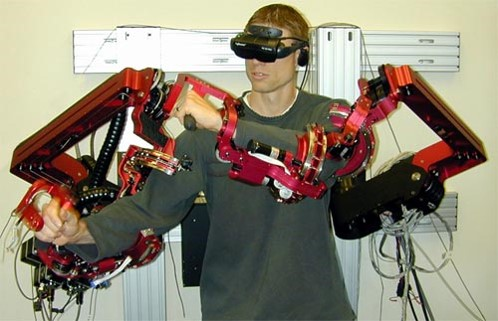
\includegraphics[width=\linewidth]{figures/ch2/ulexo}
	\caption{Figure showing a User using the \ac{ulexo} \cite{Shen2019}.}
	\label{fig:ulexo}
	%\label{key}
\end{figure}
Rehabilitation of the Upper Arm can either interact with a single arm or both arms due to the effect of the stroke, based on this definition rehabilitation robots can be classified as:
\begin{itemize}%number of arm rehabilitated
	\item \textbf{Unilateral rehabilitation}: this is the rehabilitation of only one arm/hand at a time which is usually the paretic arm \cite{Abdullah2011,Masiero2007a}.
	\item \textbf{Bilateral rehabilitation}: this is a new method that is becoming increasingly more popular with more studies showing that rehabilitating both arms together can achieve a better result faster than a unilateral therapy, and it also engages the users more,  by having them in some control modes use their more active arm to move both arms \cite{Lum1999,VanDelden2015,Wu2013,Tijs2006,Simkins2016,Shen2019a,Hsieh2016,Zhang2018,Stoykov2010}
\end{itemize}
Rehabilitation robots are built to move the impaired arm along a particular path, but in general there are some methods that are commonly used by researchers developing or using commercial robots, some of these training method/ control modes are:
\begin{itemize}\label{list:scontrol}%control modes for rehab robots
	\item \textbf{The bilateral modes of passive-passive, active-passive and active-active control modes}: this mode is seen on the \ac{mime} and \ac{arcmime} and it describes the type of activity on each arm, passive being the robot moves the arm, active being the arm has to move against a resistive force.
	\item \textbf{Master slave bilateral robot mode}: this is the control mode that is generally seen in 3D workspace rehabilitation robots, because there is no control strategy that has been seen to able to solve the problem of controlling both hands, this method makes the slave arm (connected to the paretic arm) to follow the motion of the Master arm(connected to the stronger arm) and it has been shown to work well \cite{Guo2013,Harischandra2017,Liu2010,Lott2016,Sheng2018,Shen2019a}.
	\item\textbf{ \ac{arcmime} modes of active constrained and bimanual mode}: this modes are used on both the \ac{mime} and \ac{arcmime} robots, the robots also include active and passive modes, the bimanual allows for both arms to be used for rehabilitation \cite{Mahoney2003,Waldner2009}.
	\item \textbf{Resistive and assistive rehabilitation}: this control modes describes whether the robot helps the patients to perform the task (assistive), or the robot provides a constant or varying resistive force to their action to allow them use their force (resistive). These are popular among linear planer rehabilitation robots \cite{Haghshenas-Jaryani2020,Zollo2011}.
\end{itemize}


\newpage
\subsection{Literature Review on Existing Rehabilitation robots}
Due to there being a lack of up-to-date information on Bilateral rehabilitation robots, there was a need for a literature review survey on the current state of the art in the aspect of  rehabilitation robots, that is what these reviews are aimed to solve. \\
Table \ref{tab:reviewclincal} shows details from papers from 1980 to 2020 that involved a clinical trial with a bilateral robot. Important details of note are: number of patients involved the trial. Amount of patienta within each stroke period of time, average time after stroke, intervention used, FES use involved, outcome measures used, details of intervention measures. All of which make each entry to be different from each other based on the experiment goal and patients available for testing.\\
Table \ref{tab:reviewbilateral} contains a summary of each paper reviewed and  the methods used.

\newpage
\section{Force-Torque Sensors}
\subsection{Definition of Force-Torque Sensors.}
A Force-Torque Sensor is an electronic transducers that are made up of \ac{fsr} \cite{Florez2010} that allow the transducer to be able to measure static or dynamic forces applied to its surface, through the variation of it's resistance, while a multi axis force sensor is a device that measures the outputting forces and torques from all three Cartesian coordinates (x, y, and z). A six-axis force/torque transducer is also known as a multi-axis force/torque transducer, multi-axis load cell, F/T sensor, or six-axis load cell \cite{atifts}.\\
The Importance to be able to measure all the 6 components of a generalized force is important in many testing and implementations such as force sensors for: wind tunnels, robotics, general structures \cite{Ballo2014,ATI2013,Jost2020}, with an example of commercial force sensors for general purposes shown in Figures: \ref{fig:atifs} and \ref{fig:comfs}.

\subsection{Importance of Force-Torque sensors in Rehabilitation robots.}
The need for force-sensors has been increasing due to the advances and increase in amount of human-robot interaction and robots that need to interact with humans \cite{Kim2017}. A robotic end-effector is any object attached to the robot flange (wrist) that serves a function. This includes robotic grippers, robotic tool changers, robotic collision sensors, robotic rotary joints, robotic press tooling, compliance devices, robotic paint guns, material removal tools, robotic arc welding guns, robotic transguns, etc. Robot end-effectors are also known as robotic peripherals, robotic accessories, robot tools, or robotic tools, \ac{eoa}, or end-of-arm devices \cite{atiende}.
Force-torque sensors are able to allow robots to be able to perform more functions, because of the availability of more data. This also applies to rehabilitation robots, force-torque sensors allow for the force being applied to the patient to be accurate and also allows for the force the patient applies during a active session to be recorded and used for data analysis.\\
Because the robot has to interact with a patient with usually high spasticity, there is a need to know how much the patient is actually putting into the rehabilitation process. A solution to this is to allow the patient to do most of the work and then allow the robot to only give minimal support through a resistive means \cite{Hesse2003}.\\
From the literature review (Tables:\ref{tab:reviewbilateral},\ref{tab:reviewclincal}) most authors made use of force sensors to serve 2 purposes: To measure the muscle strength of the patient, and to measure the amount of force the have they put into the rehabilitation process. And it also helps to monitor the force levels applied to the patients, so they don’t become dangerous \cite{Adamovich2009,Diez2018}.
\begin{figure}[p]%ati loadcell image
	\centering
	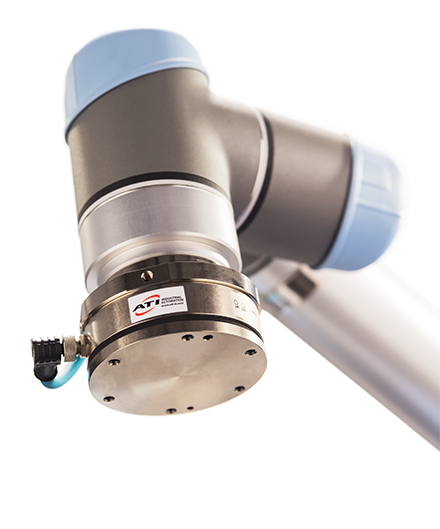
\includegraphics[height=0.5\textheight]{figures/ch2/ati}
	\caption{Figure showing an ATI force-sensor attached to the end of a \ac{ur}5 robot system \cite{atipiclink}.}
	\label{fig:atifs}
\end{figure}

\begin{figure}[p]%commercial load cell image
	\centering
	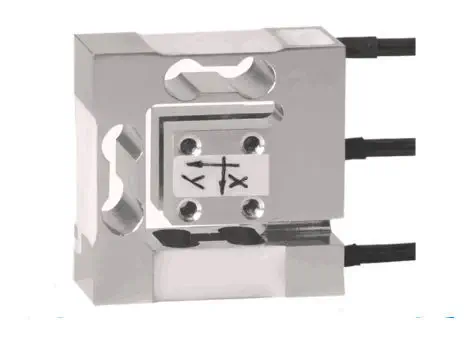
\includegraphics[width=12cm]{figures/ch2/commercialloadcell}
	\caption{Figure showing a Commercial 3-axis Force Sensor.}
	\label{fig:comfs}
\end{figure}

\newpage
\section{Transfer Learning}
\subsection{What is Transfer Learning?}
Transfer Learning or knowledge transfer are algorithm methods that are used to reduce the need and effort to recollect training data to solve multiple problems between different task domains \cite{Pan2010}.\\
From \cite{Pan2010} Transfer Learning is defined in definition \ref{def:tf}
\begin{dft}{\textbf{Transfer Learning.}}\label{def:tf}
	Given a source domain $\mathcal{D}_{\mathcal{S}}$ and a learning task $\mathcal{T}_{\mathcal{S}}$,a Target Domain $\mathcal{D}_{\mathcal{T}}$ and learning task $\mathcal{T}_{\mathcal{T}}$, transfer learning aims to help improve the learning of the target predictive function $f_{T}(.)$ in $\mathcal{D}_{T}$  using the knowledge in $\mathcal{D}_{\mathcal{S}}$ and $\mathcal{T}_{\mathcal{S}}$, where $\mathcal{D}_{\mathcal{S}}~ \neq~ \mathcal{D}_{\mathcal{T}}$ or  $\mathcal{T}_{\mathcal{S}}~\neq~ \mathcal{T}_{\mathcal{T}}$.
\end{dft}
This definition describes a situation whereby a particular problem is solved in a particular domain using a machine learning model, can we then take some of the knowledge obtained from the known model to reduce the training time for the new time by making use of the relationship between either, the problem domain, data domain and data relationship.

\subsection{Uses for Transfer Learning}
Many machine learning methods only work well only under a common assumption, which is that both the training and test data are drawn from the same feature space and distribution \cite{Pan2010}. This leads to models needing to be rebuilt using new data if the distribution or the feature space changes, which can be very expensive or impossible to get all the new data require. In such cases Transfer Learning between Domains would be desirable.\\

\subsection{Categories of Transfer Learning}
Based on the three main research issues of transfer learning: what to transfer?, how to transfer? and when to transfer? \cite{Pan2010}.
For when to transfer?, this is dependent on the problem to be solve and whether there is a need for transfer e.g. dealing with large data or lack of suitable data, that determines a need for transfer learning.\\ 
Transfer learning can be categorized based on each of the three research areas, the categorized will be described in the sections below:

\subsubsection{What to transfer?}
On the aspect of `What to Transfer?', this section is concerned with what part of the knowledge can be transferred across domains. Based on the definition above there are 4 cases for which we can choose a parameter from a model to transfer to another model \cite{Pan2010}, and these are:
\begin{itemize}
	\item[Instance ] This method assumes that some part of the data in the source domain can be reused in the target domain by re-weighting and importance sampling \cite{Pan2010,Xu2018,Cortes2007,Xia2013,Rohrbach2013,Zhang2010}.
	\item[Feature-representation] In this case, the idea is to learn a `good' representation for the target domain, meaning the knowledge to be transferred is encoded into the learned feature representation to improve performance \cite{Pan2010,Kandaswamy2014,Xia2013,Niu2021,Bahadori2014,Pan2008}. 
	\item[Parameter] In this scenario it is assumed both the source and target task share some parameters or distribution of the hyper-parameters of the models, the knowledge to be transferred is encoded into the shared parameters or priors, therefore by finding the shared parameters between domains it can be successfully be transferred \cite{Pan2010,Kumagai2016,Denil2013,Houlsby2019,Huang2010,Chapelle2000}.
	\item[Relational-knowledge] This method is similar to the parameter transfer method, but here  it is the data for both the source and target domain that are similar, therefore the knowledge to be transferred is the relationship between the data, statistical techniques are the most dominant in this field \cite{Pan2010,Niu2021,Yao2010,Tang2013,Rossi2018,Ramon2007}.
\end{itemize}

\subsubsection{How to Transfer?}
Based off the definition of transfer learning and the information from the section, transfer learning can be categorized into 3, inductive, transductive and unsupervised transfer learning, describing each in more detail below:
\begin{itemize}
	\item[Inductive ] in this scenario the source and target tasks will always be different, even though their domains might be similar, labelled data from the source is needed to induce a model for the target domain. Based on the amount of unlabelled data in the source domain this scenario can be further split into 2 cases: self-taught learning and multitask learning shown in Figure \ref{fig:pantl} \cite{Pan2010}.
	\item[Transductive] in this scenario compared to the one above, the tasks are the same, while the domains are not, it is assumed here that there is no labelled data in the target domain while there is plenty in the source domain. this scenario can be further split into 2 shown in Figure \ref{fig:pantl} which are Domain Adaptation and sample selection bias/covariance shift \cite{Pan2010}.
	\item[Unsupervised] this form is similar to the Inductive transfer learning, except it is used for solving unsupervised learning tasks in the target domain such as clustering, dimensionality reduction and density estimation \cite{Pan2010}.
\end{itemize}
\begin{figure}[p]
	\centering
	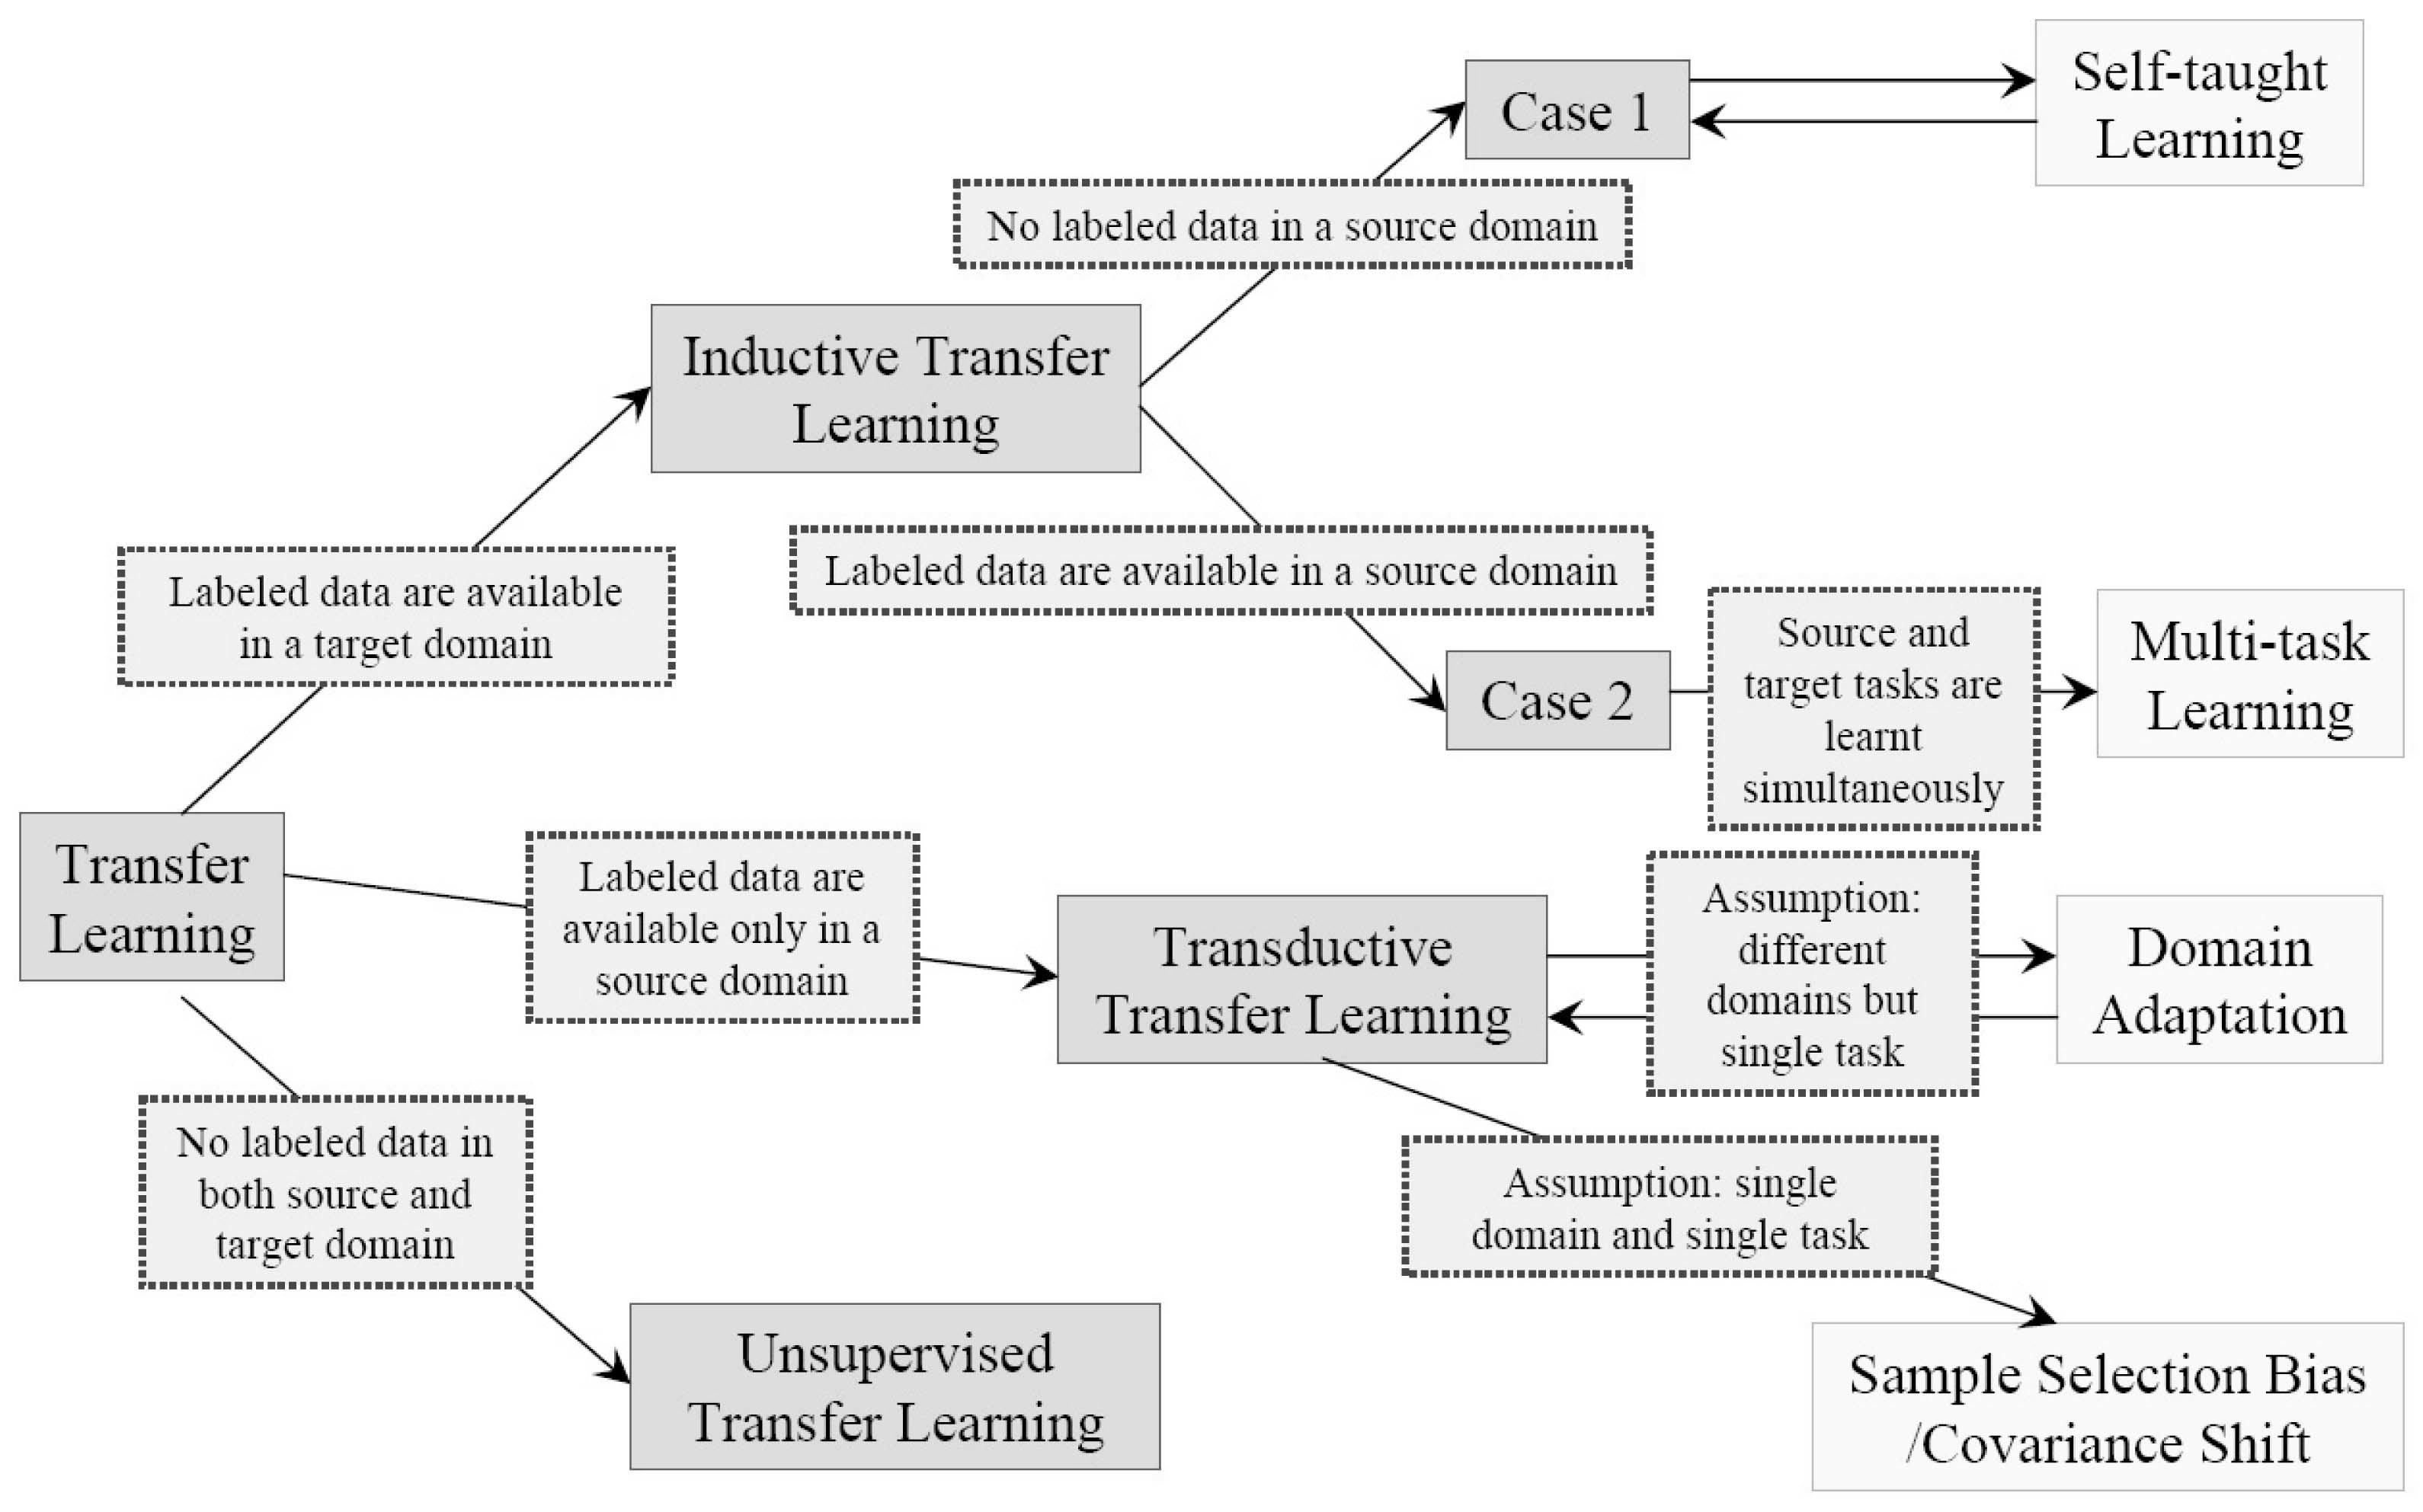
\includegraphics[width=1.1\linewidth]{figures/ch2/pantl}
	\caption{Figure showing the specification that lead to the choice of Transfer learning methods \cite{Pan2010}.}
	\label{fig:pantl}
\end{figure}